\chapter{\RU{Числа Фибоначчи}\EN{Fibonacci numbers}}

\RU{Еще один часто используемый пример в учебниках по программированию это рекурсивная ф-ция,
генерирующая числа Фибоначчи}
\EN{Another often used in programming textbooks example is a recursive function 
generating Fibonacci numbers}\footnote{\url{http://oeis.org/A000045}}.
\RU{Последовательность очень простая: каждое следующее число это сумма двух предыдущих}\EN{The 
sequence is very simple: each consecutive number is a sum of two previous}.
\RU{Первые два числа это единицы или 0, 1 и 1}\EN{First two numbers are 1's or 0, 1 and 1}.

\RU{Начало последовательности}\EN{The beginning of the sequence is}:

\begin{center}
$0, 1, 1, 2, 3, 5, 8, 13, 21, 34, 55, 89, 144, 233, 377, 610, 987, 1597, 2584, 4181 ...$
\end{center}

\section{\RU{Пример}\EN{Example} \#1}

\RU{Реализация проста. Эта программа генерирует последовательность вплоть до}
\EN{Implementation is simple. This program generates a sequence till} 21.

\lstinputlisting{patterns/208_fib/fib.c}

\lstinputlisting[caption=MSVC 2010 x86]{patterns/208_fib/fib.asm}

\RU{Этим я хотел проиллюстрировать стековые фреймы}\EN{So I wanted to illustrate 
stack frames by this}.
\RU{Загрузим пример в \olly и дотрассируем до самого последнего вызова ф-ции f()}
\EN{Let's load the example to \olly and trace to the latest call of f() function}:
\figref{fig:fib_olly}.

\RU{Исследуем стек более пристально}\EN{Let's investigate stack more closely}. 
\RU{Я добавил здесь комментариев}\EN{I added some comments to it}
\footnote{\EN{By the way, it's possible to select several entries in \olly and copy them to clipboard (Ctrl-C).
That's what I just did.}\RU{Кстати, в \olly можно отметить несколько элементов и скопировать их
в клипбоард (Ctrl-C). Я это только что сделал}}:

\lstinputlisting{patterns/208_fib/stack.txt}

\RU{Ф-ция рекурсивная}\EN{The function is recursive}
\footnote{\RU{т.е., вызывающая сама себя}\EN{i.e., calling itself}}, 
\RU{поэтому стек выглядит как ``бутерброд''}\EN{hence stack looks like ``sandwich''}.
\RU{Мы видим что аргумент}\EN{We see that} \IT{limit} \RU{всегда один и тот же}
\EN{argument is always the same} (\TT{0x14} \OrENRU 20), \RU{но аргументы}\EN{but} \IT{a} 
\AndENRU \IT{b} \RU{разные при каждом вызове}\EN{arguments are different for each call}.
\RU{Здесь также адреса \ac{RA} и сохраненные значения \EBP}
\EN{There are also \ac{RA}-s and saved \EBP values}.
\olly \RU{способна определять EBP-фреймы, так что она тут нарисовала скобки}
\EN{is able to determine EBP-based frames, so it draws these brackets}.
\RU{Значения внутри каждой скобки это \gls{stack frame}, иными словами, место, которое каждая
инкарнация ф-ции может использовать для любых своих нужд}\EN{Values inside of each bracket 
are \gls{stack frame}, 
in other words, stack area which each function incarnation can use as scratch space}. 
\RU{Можно сказать, каждая инкарнация ф-ции не должна обращаться к элементам стека за пределами
фрейма (не учитывая аргументов ф-ции), хотя это и возможно технически}
\EN{We can also say that each function incarnation must not access
stack elements beyond frame boundaries (excluding function arguments), 
although it's technically possible}. 
\RU{Обычно это так и есть, если только ф-ция не содержит каких-то ошибок}
\EN{It's usually true, unless function has bugs}.
\RU{Каждое сохраненное значение \EBP это адрес предыдущего \gls{stack frame}:
это причина, почему некоторые отладчики могут легко делить стек на фреймы и выводить
аргументы каждой ф-ции.}
\EN{Each saved \EBP value is an address of previous \gls{stack frame}: 
it is a reason why some debuggers can easily divide stack by frames and dump each 
function's arguments.}
% FIXME add about StackWalk (MSDN)

\RU{Как видно, каждая инкарнация ф-ции готовит аргументы для следующего вызова ф-ции}
\EN{As we see here, each function incarnation prepares arguments for the next function call}.

\RU{В самом конце мы видим 3 аргумента ф-ции}\EN{At the very end we see a 3 arguments for} \main. 
\TT{argc} \RU{равен}\EN{is} 1 (\RU{да, действительно, я запустил эту программу
без аргументов в командной строке}\EN{yes, indeed, the program I run without command-line 
arguments}).

\RU{Очень легко устроить переполнение стека: просто удалите (или закомментируйте) проверку
предела и процесс упадет с исключением}
\EN{It's easy to do stack overflow: just remove (or comment) limit check and it will crash with
exception} \TT{0xC00000FD} (\RU{переполнение стека}\EN{stack overflow}).

\begin{figure}[H]
\centering
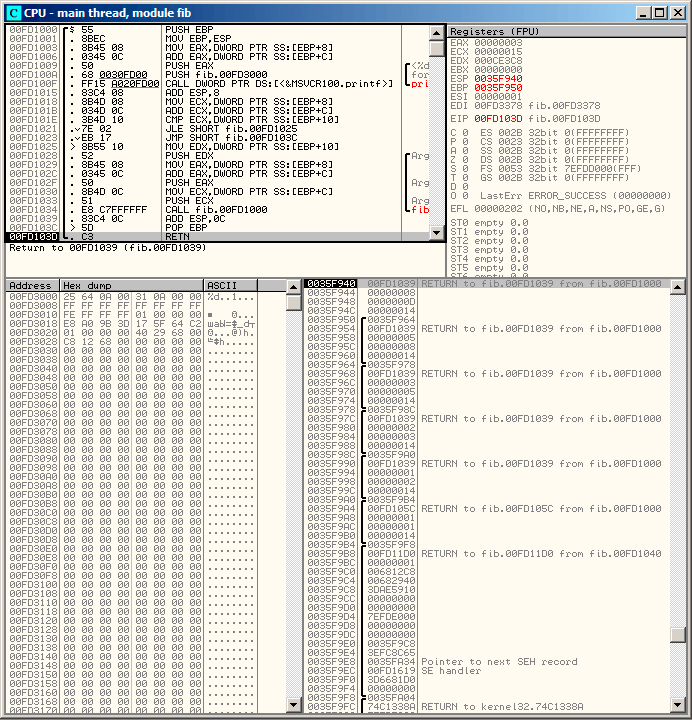
\includegraphics[scale=\FigScale]{patterns/208_fib/olly.png}
\caption{\olly: \RU{последний вызов f()}\EN{last call of f()}}
\label{fig:fib_olly}
\end{figure}

\section{\RU{Пример}\EN{Example} \#2}

\RU{В моей ф-ции есть некая избыточность, так что добавим переменную \IT{next} и заменим на нее
все ``a+b''}
\EN{My function has some amount of redundancy, so let's add new local variable \IT{next} and 
replace all ``a+b'' by it}:

\lstinputlisting{patterns/208_fib/fib2.c}

\RU{Это результат работы неоптимизирующего MSVC, поэтому переменная \IT{next} действительно
находится в локальном стеке}
\EN{This is output of non-optimizing MSVC, so \IT{next} variable is actually allocated 
in local stack}:

\lstinputlisting[caption=MSVC 2010 x86]{patterns/208_fib/fib2.asm}

\RU{Загрузим}\EN{Let's load} \olly \RU{снова}\EN{again}: \figref{fig:fib_olly2}.
\RU{Теперь переменная \IT{next} присутствует в каждом фрейме}
\EN{Now \IT{next} variable is present in each frame}.

\RU{Рассмотрим стек более пристально. Я снова добавил туда своих комментариев}
\EN{Let's investigate the stack more closely. I added my comments again}:

\lstinputlisting{patterns/208_fib/stack2.txt}

\RU{Значение переменной \IT{next} вычисляется в каждой инкарнации ф-ции, затем передается
аргумент \IT{b} в следующую инкарнацию} % FIXME what a word! hmmm...
\EN{Here we see it: \IT{next} value is calculated in each function incarnation, then passed as
\IT{b} argument to the next incarnation}.

\begin{figure}[H]
\centering
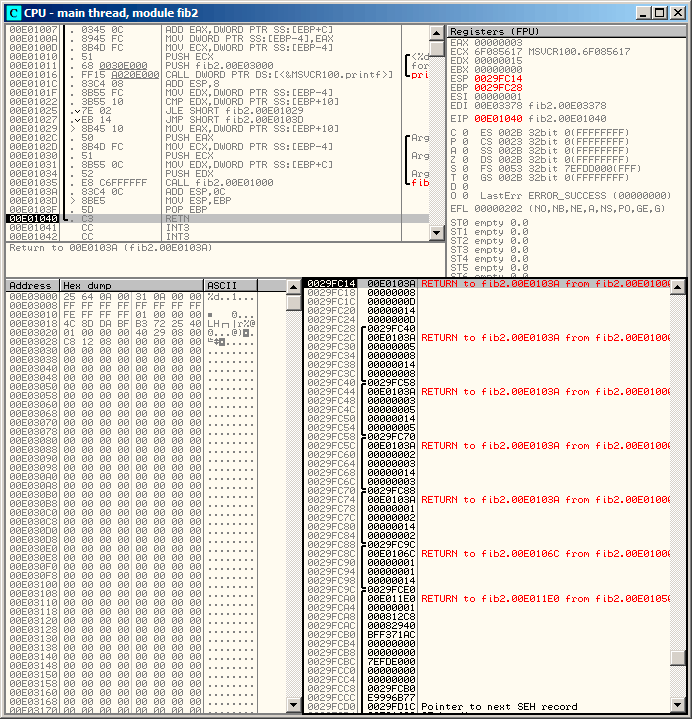
\includegraphics[scale=\FigScale]{patterns/208_fib/olly2.png}
\caption{\olly: \RU{последний вызов f()}\EN{last call of f()}}
\label{fig:fib_olly2}
\end{figure}

\section{\RU{Итог}\EN{Summary}}

% FIXME: add \index{recursion}
\RU{Рекурсивные ф-ции эстетически красивы, но технически могут ухудшать производительность
из-за активного использования стека}
\EN{Recursive functions are \ae{}sthetically nice, but technically may degrade performance because
of heavy stack usage}.
\RU{Тот, кто пишет критические к времени исполнения участки кода, наверное, должен избегать 
применение там рекурсии}\EN{One who write performance critical code pieces, probably, 
should avoid recursion there}.
